% !TeX spellcheck = it_IT
\newpage
\section{Performance}
Un modello per misurare le performance di un sistema ICT è il seguente:
\begin{center}
	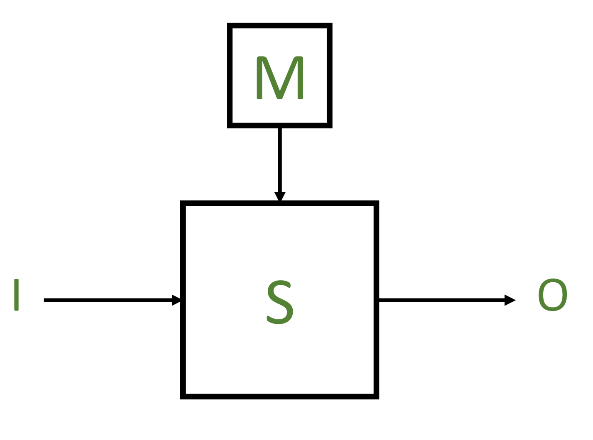
\includegraphics[scale=0.3]{performance_model.png}
\end{center}
in cui abbiamo degli \textbf{input} elaborati dal sistema che produce \textbf{output} è che viene monitorato per la \textbf{QoS} (Quality of Service) da un \textbf{monitor}.\\
Il \textbf{monitoraggio} di metriche di performance in un sistema ICT è fondamentale per garantirne il corretto funzionamento e necessita quindi di un \textbf{modello}. Queste metriche devono essere messe in corrispondenza con una \textbf{Quality of Service} da garantire, e viene fatto nel \textbf{Service Level Agreement} (SLA).

\subsection{Metriche}
\begin{definition}[Metrica]
	Si tratta della misurazione di una caratteristica (o di un insieme di esse) di un sistema che fornisce un'informazione utile.
\end{definition}
In sistemi complessi le metriche possono essere combinate mediante:
\begin{itemize}
	\item \textbf{Somma} (e.g. latenza)
	\item \textbf{Moltiplicazione} (e.g. disponibilità)
	\item \textbf{Max/Min} (e.g banda)
\end{itemize}

\subsubsection{Categorie}
Le metriche di performance di un sistema ICT si dividono in 4 categorie:
\begin{itemize}
	\item \textbf{Elaborazione} 
	\begin{itemize}
		\item \emph{Capacità di calcolo}: il massimo numero di richieste per unità di tempo che il sistema riesce a processare senza perdite
		\item \emph{Qualità}: la precisione ottenuta dai risultati
	\end{itemize}
	\item \textbf{Trasmissione} dati
	\begin{itemize}
		\item \emph{Banda}: il massimo throughput di dati supportato da un collegamento all'altro o lungo un cammino nella rete. La \emph{banda disponibile} si ottiene come differenza tra la \emph{banda nominale} e quella attualmente in uso
		\item \emph{Latenza}:  l’intervallo di tempo in cui si completa il trasferimento di dati
		lungo un collegamento o un cammino di rete
		\item \emph{Jitter}: la variazione di latenza tra richieste successive
		\item \emph{Packet loss}: la percentuale di pacchetti non ricevuti sul totale di
		pacchetti inviati
	\end{itemize}
	\item \textbf{Immagazzinamento} dati
	\begin{itemize}
		\item \emph{Capacità}: spazio a disposizione per salvare i dati
		\item \emph{Throughput}: massima quantità di dati che si riescono a
		scrivere/leggere per unità di tempo
	\end{itemize}
	\item \textbf{Qualità dell'esperienza} dell'utente. Spesso riportata su una scala da 1 a 5 e può includere \emph{disponibilità}, \emph{framerate}, \emph{qualità video}, etc.
\end{itemize}
\subsection{Efficienza energetica}
Dato il modello in precedenza, aggiungiamo l'\textbf{energia elettrica} utilizzata e l'\textbf{anidride carbonica} prodotta:
\begin{center}
	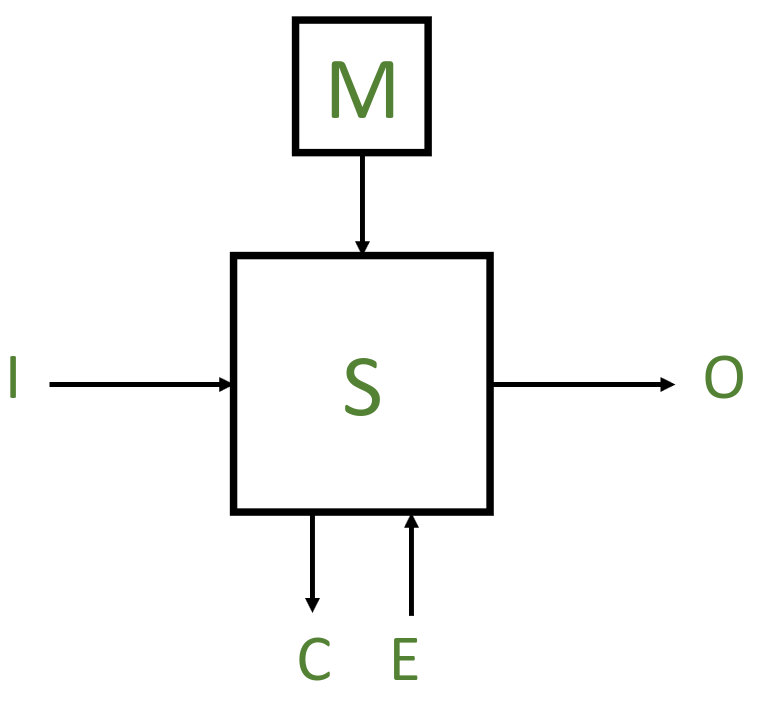
\includegraphics[scale=0.2]{performance_model_energy.png}
\end{center}
Un primo modo per valutare un sistema ICT dal punto di vista \emph{energetico} è tramite l'\textbf{efficienza}:
\begin{equation}
	\epsilon = \frac{\#calcoli}{E}=\bigg[\frac{FLOPS}{J}\bigg] \simeq \bigg[\frac{FLOPS}{W}\bigg]
\end{equation}

\begin{definition}[Legge di Koomey]
	La quantità di calcoli per Joule di energia raddoppia all'incirca ogni $1.5$ anni.
\end{definition}
La legge si è dimostrata vera fino al 2010 circa. Oggi raddoppia ogni $2.5$ anni si fermerà come quella di Moore e quella di Dennard.\\
Allo stesso modo la quantità di batteria necessaria per svolgere una certa quantità di calcoli diminuisce nel tempo (oggi di 16 volte ogni 10 anni).

\subsubsection{Power Usage Effectiveness}
L'energia consumata nel mondo ICT si divide in:
\begin{itemize}
	\item Per i \textbf{sistemi IT}
	\begin{itemize}
		\item Energia per alimentare server e dispositivi di rete
	\end{itemize}
	\item Per i \textbf{sistemi non IT}
	\begin{itemize}
		\item Sistemi di raffreddamento
		\item Sistemi di allarme e UPS
		\item Sistemi di illuminazione
	\end{itemize}
\end{itemize}
Per valutare l'efficienza di un sistema ICT si usa il Power Usage Effectiveness (PUE):
\begin{equation}
	PUE=\frac{P_{IT}+P_{non-IT}}{P_{IT}} = 1+\frac{P_{non-IT}}{P_{IT}}
\end{equation}

\subsubsection{Datacentre Infrastructure Efficiency}
L'inverso del PUE è detto Datacentre Infrastructure Efficiency (DCiE):
\begin{equation}
	DCiE=\frac{P_{IT}}{P_{IT}+P_{non-IT}}=\frac{1}{PUE}
\end{equation}

\newpage
Sia PUE che DCiE sono influenzati da:
\begin{itemize}
	\item \textbf{Utilizzo} del sistema nel \emph{tempo} e nello \emph{spazio}
	\item \textbf{Età} e \textbf{progettazione} del sistema
	\item \textbf{Efficienza} complessiva del sistema
\end{itemize}
Alcuni valori tipici sono:
\begin{table}[h]
	\centering
	\begin{tabular}{|c|c|c|}
		\hline
		\textbf{PUE} & \textbf{DCiE} & \textbf{Level of Efficiency} \\
		\hline
		$3.0$ & $33\%$ & Very inefficient \\
		\hline
		$2.5$ & $40\%$ & Inefficient \\
		\hline
		$2.0$ & $50\%$ & Average \\
		\hline
		$1.5$ & $67\%$ & Efficient \\
		\hline
		$1.2$ & $83\%$ & Very efficient \\
		\hline
	\end{tabular}
\end{table}